\section{Let Míčku}
\label{sec:let-micku}
Let míčku se často zjednodušuje a zanedbávají se některé síly, které na letící
míček působí. Když uvážíme jen gravitaci zjistíme, že by míček za letu měl
dráhou opsat parabolu. Pro kratší dobu letu a velkou rychlost tento předpoklad
není nikterak škodlivý.\footnote{Jako tomu bývá často právě ve stolním tenisu}.
Tyto síly můžeme vidět na rovnici \myref{rovnici}{eq:Newton} a na
\myref{obrázku}{fig:let-micku}.

\myref{Rovnice}{eq:Newton} získáme, když si rozepíšeme 2. Newtonův kinematický
zákon. 
\begin{equation}
 \label{eq:Newton}
 \speed{} + \textcolor{teal}{\vec{F_g}} +
 \textcolor{drcol}{\vec{F_d}} + \textcolor{spcol}{\vec{F_m}} = m \vec{a}
\end{equation}
Kde:
\begin{itemize}
  \item[$\speed{}$] Rychlost
  \item[$\textcolor{teal}{\vec{F_g}}$] Gravitace
  \item[$\textcolor{drcol}{\vec{F_d}}$] Odpor vzduchu (anglicky \uv{drag})
  \item[$\textcolor{spcol}{\vec{F_m}}$] Magnusova síla
\end{itemize}

Síly působící na letící míček v průběhu budou podrobněji popsané dále v této
sekci.

\begin{figure}[htbp]
 \centering
 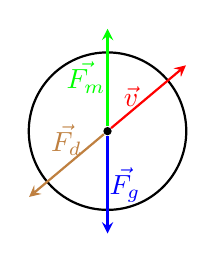
\begin{tikzpicture}
	%giganteska bola de fuego
	\node[fill=black,circle,inner sep=0pt, minimum size=3pt](center) at (0,0)
	{};
 \draw[thick] (center) circle (1);


	%speed
	\draw[thick, red, -stealth] (center) -- node[midway, left] {$\vec{v}$} (40:1.3);

	%gravitace
	\draw[thick, blue, -stealth] (center) --node[midway,right=-3pt] {$\vec{F_g}$} (-90:1.3);

	%drag
	\draw[thick,brown, -stealth] (center) --node[midway,left,above] {$\vec{F_d}$}
	 (220:1.3);

	%magnus force
	\draw[thick,green,-stealth] (center) --node[left=-3pt,midway] {$\vec{F_m}$} (90:1.3);


\end{tikzpicture}


 \caption{Síly působící na míček v letu}
 \label{fig:let-micku}
\end{figure}


\subsection{Rychlost}
\label{ssec:rychlost}
Rychlost ($\speed{}$), jako derivace polohy je jádrem samotného pohybu
(bez změny polohy není pohyb). Ze začátku dáme míčku nějakou energii a tím ho
uvedeme v pohyb.

Jakmile je ve vzduchu, působí na něj ostatní síly a ovlivňují jeho energii.
V případě, kterým se budeme zabívat, většina sil disipuje energii míčku. Jediný
jev, který by mohla prodlužovat dobu letu (tedy přidávat míčku energii) je jev
Magnusův. Tomu je věnována \myref{podsekce}{ssec:magnusova-sila}.


\subsection{Gravitační síla}
\label{ssec:gravitacni-sila}

Gravitační a v tomto případě můžeme říci i tíhová síla\footnote{Gravitační a
 tíhová jsou obecně odlišné síly a v některých případech je nutné je tak vnímat. Toto ovšem
není jeden z nich proto je můžeme
zaměnit.\autocite{reichlEncyklopedieFyziky2006} Dále bude používán jen termín
gravitační síla.} (\textcolor{grcol}{$F_g$}) je hned po rychlosti
nejdůležitější sílou v průběhu pohybu míčku. A spolu s rychlostí nejviditelněji
tvoří trajektorii míčku.

Gravitace je také nejednoduší na modelování. Dokud můžeme pro celou trajektorii
považovat Zemi za lokálně plochou, gravitační síla míří vždy směrem kolmo dolů.
Také její amplituda bývá většinou konstantní, protože není časté, že by míček
během letu měnil svojí hmotnost a gravitační zrychlení se také nemění.

Matematicky můžeme z 2. Newtonova zákona velikost gravitační síly vyjádřit
jako:
\[
 \textcolor{grcol}{F_g} = mg
\]
Kde $g$ je gravitační zrychlení (často zaokrouhlováno na $10~m/s$) a $m$ je
hmotnost míčku.

Z této rovnice je ještě jednodušší nahlédnout na fakt, že gravitační síla je pro
náš případ konstantní. 


\subsection{Odpor vzduchu}
\label{ssec:odpor-vzduchu}

Odpor vzduchu (\textcolor{drcol}{$F_d$}) si můžeme dovolit zanedbat, protože
zkoumáme jen velmi krátký let. Kdyby se jednalo například o dlouhé odpaly v
baseballu, tehdy již odpor vzduchu zanedbatelný není.

Na rozdíl od gravitační síly, odpor vzduchu není konstantní v průběhu letu. Odpor
vzduchu je totiž obecně závislí na rychlosti a ploše, která aktivně do vzduchu
naráží. V případě koule se mění jen rychlost. Což o hodně zjednodušuje výsledný
výpočet. 

Směr odporu vzduchu je vždy opačný ke směru pohybu jak můžeme vidět na
\myref{obrázku}{fig:let-micku}. Velikost odporu závisí 
kromě dalších koeficientů hlavně na kvadrátu rychlosti. 


\subsection{Magnusova síla}
\label{ssec:magnusova-sila}

Magnusova síla (\textcolor{spcol}{$F_m$}) vzniká díky rotaci a vzájemnému tření
mezi míčkem a vzduchem (předpokládáme vzduch bez vlastní rychlosti). Intuitivním
vysvětlením tohoto fenoménu je, že rotací a třením se vzduch posouvá po směru
rotace, a z 3. Newtonova zákona plyne, že vzduch by měl opačnou silou působit
zpět. Magnusův efekt je znát pouze je-li hmotnost míčku dostatečně malá nebo
úhlová rychlost dostatečně
velká.\autocite{universityMagnusEffectThermodynamics}

Směr $\textcolor{spcol}{\vec{F_m}}$ na \myref{obrázku}{fig:let-micku} je specifický pro aktuální
případ.\footnote{Předpokládáme pouze backspin, jak bude zmíněno v kapitole
[triviální případy] je to jedna z podmínek zpětného odrazu.} Směr Magnusovi síly
závisí na úhlové rychlost ($\spin{1}$). Nejen svojí velikostí, ale i směrem.
Jestliže $\spin{1}<0$ tak Magnusova síla míří směrem nahoru a v opačném případě
dolů.\autocite{AerospaceMicroLesson22}
